\documentclass{homework}

\usepackage{minted}
\usepackage{tikz}
\usetikzlibrary{graphs, graphs.standard}

\title{
    15-415/615 - Database Applications

    Answers to Homework 8
}
\author{Shangning Xu}

\begin{document}

\maketitle

\section{Serializability and 2PL}

\begin{enumerate}
    \item \begin{enumerate}
        \item Yes
        \item Yes
        \item Yes
        \item No
        \item No
    \end{enumerate}

    \item \begin{enumerate}
        \item No
        \item 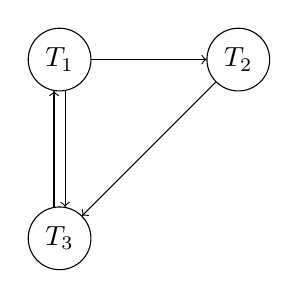
\begin{tikzpicture}
            \node [draw, circle] (T1) at (0,0) {$T_1$};
            \node [draw, circle] (T2) at (15ex,0) {$T_2$};
            \node [draw, circle] (T3) at (0,-15ex) {$T_3$};

            \draw [->] (T1) -- (T2);
            \draw [->] (T2) -- (T3);
            \draw [->] (node cs:name=T1, angle=-80) -- (node cs:name=T3, angle=80);
            \draw [->] (node cs:name=T3, angle=100) -- (node cs:name=T1, angle=-100);
        \end{tikzpicture}
        \item No
        \item No
        \item Because there are two cycles $T_1 \to T_3 \to T_1$ and $T_1 \to T_2 \to T_3 \to T_1$ in the precedence graph.
        \item No
    \end{enumerate}
\end{enumerate}

\section{Deadlock Detection and Prevention}

\begin{enumerate}
    \item \begin{enumerate}
        \item \begin{tabular}{|c||c|c|c|c|c|c|c|}
            \hline
            time & $t_1$ & $t_2$ & $t_3$ & $t_4$ & $t_5$ & $t_6$ & $t_7$ \\ \hline\hline
            LM   & g     & g     & g     & g     & b     & b     & g     \\ \hline
        \end{tabular}
        \item \tikz [nodes={draw, circle}] \graph {
            subgraph I_n [clockwise=\tikzgraphVnum, math nodes, V={T_1, T_2, T_3}];
            T_3 -> T_2 -> T_1;
        };
        \item There is no deadlock as the wait-for graph is acyclic.
    \end{enumerate}

    \item \begin{enumerate}
        \item \begin{tabular}{|c||c|c|c|c|c|c|c|c|}
            \hline
            time & $t_1$ & $t_2$ & $t_3$ & $t_4$ & $t_5$ & $t_6$ & $t_7$ & $t_8$ \\ \hline\hline
            LM   & g     & g     & g     & b     & g     & b     & b     & b     \\ \hline
        \end{tabular}

        \item There is a deadlock in the requests as there is a cycle in the wait-for graph below.
        
        \tikz [nodes={draw, circle}] \graph {
            subgraph I_n [clockwise=\tikzgraphVnum, math nodes, V={T_1, T_3, T_2, T_4}];
            T_1 -> T_4 -> T_2 -> T_3 -> T_1;
        };

        \item \begin{tabular}{|c||c|c|c|c|c|c|c|c|}
            \hline
            time & $t_1$ & $t_2$ & $t_3$ & $t_4$ & $t_5$ & $t_6$ & $t_7$ & $t_8$ \\ \hline\hline
            LM   & g     & g     & g     & a $T_1$     & g     & a $T_2$     & g     & g     \\ \hline
        \end{tabular}

        \item \begin{tabular}{|c||c|c|c|c|c|c|c|c|}
            \hline
            time & $t_1$ & $t_2$ & $t_3$ & $t_4$ & $t_5$ & $t_6$ & $t_7$ & $t_8$ \\ \hline\hline
            LM   & g     & g     & g     & b     & g     & b     & a $T_1$     & a $T_2$     \\ \hline
        \end{tabular}
    \end{enumerate}
\end{enumerate}

\section{Hierarchical Locking - Return of Bike Sharing}

\begin{enumerate}
    \item $\mathbf{IS}(D)$, $\mathbf{S}(T)$
    \item $\mathbf{IX}(D)$, $\mathbf{IX}(B)$, $\mathbf{S}(B_{10}, B_{12}\textrm{--}B_{70})$, $\mathbf{SIX}(B_{11})$, $\mathbf{X}(B_{11}:44)$
    \item $\mathbf{IX}(D)$, $\mathbf{X}(T)$
    \item $\mathbf{IX}(D)$, $\mathbf{SIX}(T)$, $\mathbf{X}(B_i: j)$ for $j$th ($1 \le j \le 100$) record in $i$th ($1 \le i \le 150$) page whose \texttt{start\_city} attribute is `Pittsburgh.'
    \item $\mathbf{X}(D)$
\end{enumerate}

\end{document}
